\documentclass{beamer}

\usepackage[utf8]{inputenc}
\usepackage[T1]{fontenc}
\usepackage[english]{babel}
\usepackage{lmodern}

\usetheme{UOS}

\graphicspath{{images/}}

\renewcommand{\baselinestretch}{1.25}

\begin{document}

\title{Normal Calculation in Point Clouds with CUDA}
\author[Matthias Greshake, Alexander Mock]{Matthias Greshake, Alexander Mock\\ {\scriptsize mgreshake@uos.de, amock@uos.de}}
\institute{Institut für Informatik\\ AG Wissensbasierte Systeme}
\date{26. January 2016}

\begin{frame}[plain]
	\titlepage
\end{frame} 

\begin{frame}{Outline}
	\tableofcontents
\end{frame} 

\section{Motivation}
\begin{frame}{Motivation}
  %Pointcloud und optimiertes Mesh untereinander/nebeneinander
  %vielleicht auch hintereinander/voreinander
\end{frame}

\subsection*{Point Clouds}
\begin{frame}{Point Clouds}
 
    
  \begin{columns}
  
   \begin{column}{0.55\textwidth}
   
    \begin{figure}
      \centering
      
      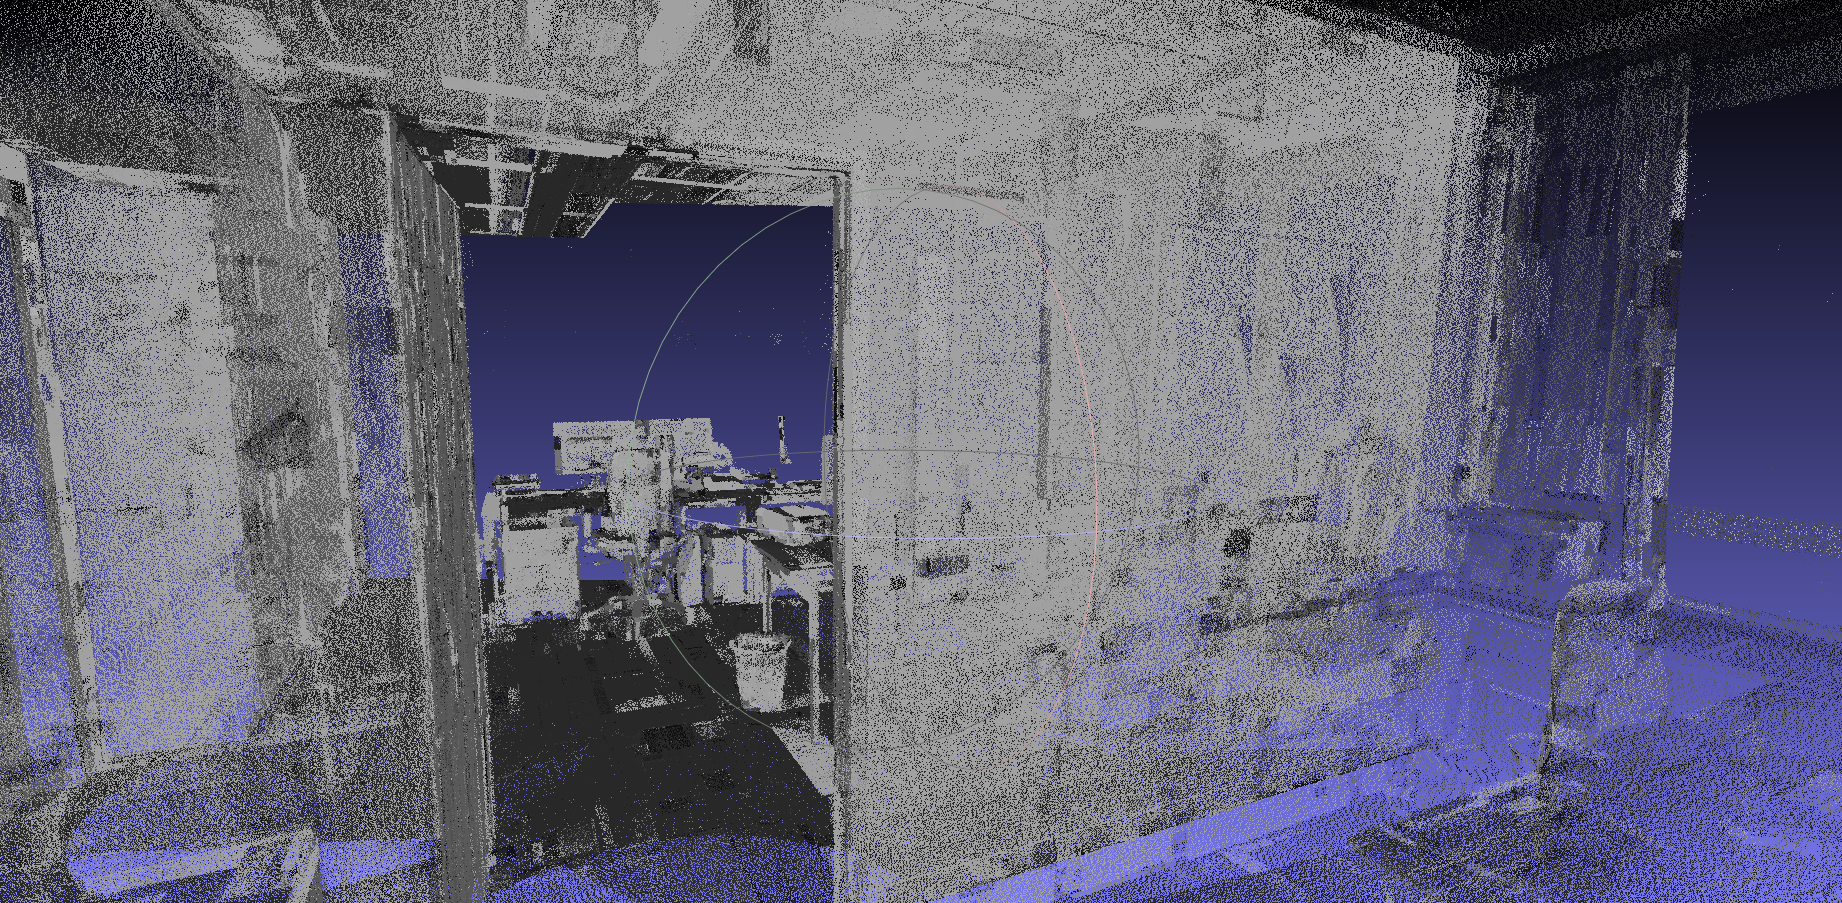
\includegraphics[width=1.0\linewidth]{Images/police_points.png}
   
    \end{figure}
    
    
   \end{column}
  \begin{column}{0.45\textwidth}
  
   \begin{itemize}
    \item Depth sensors: 3D Laserscanner
    \item High number of points 
    \item No topological information between points
    \item Fit a memory minimized polygonmesh
    
   \end{itemize}
  \end{column}

   
  \end{columns}
 
\end{frame}

\subsection*{Reconstruction}
\begin{frame}{Reconstruction}
 
    
  \begin{columns}
  
   \begin{column}{0.55\textwidth}
   
    \begin{figure}
      \centering
   
      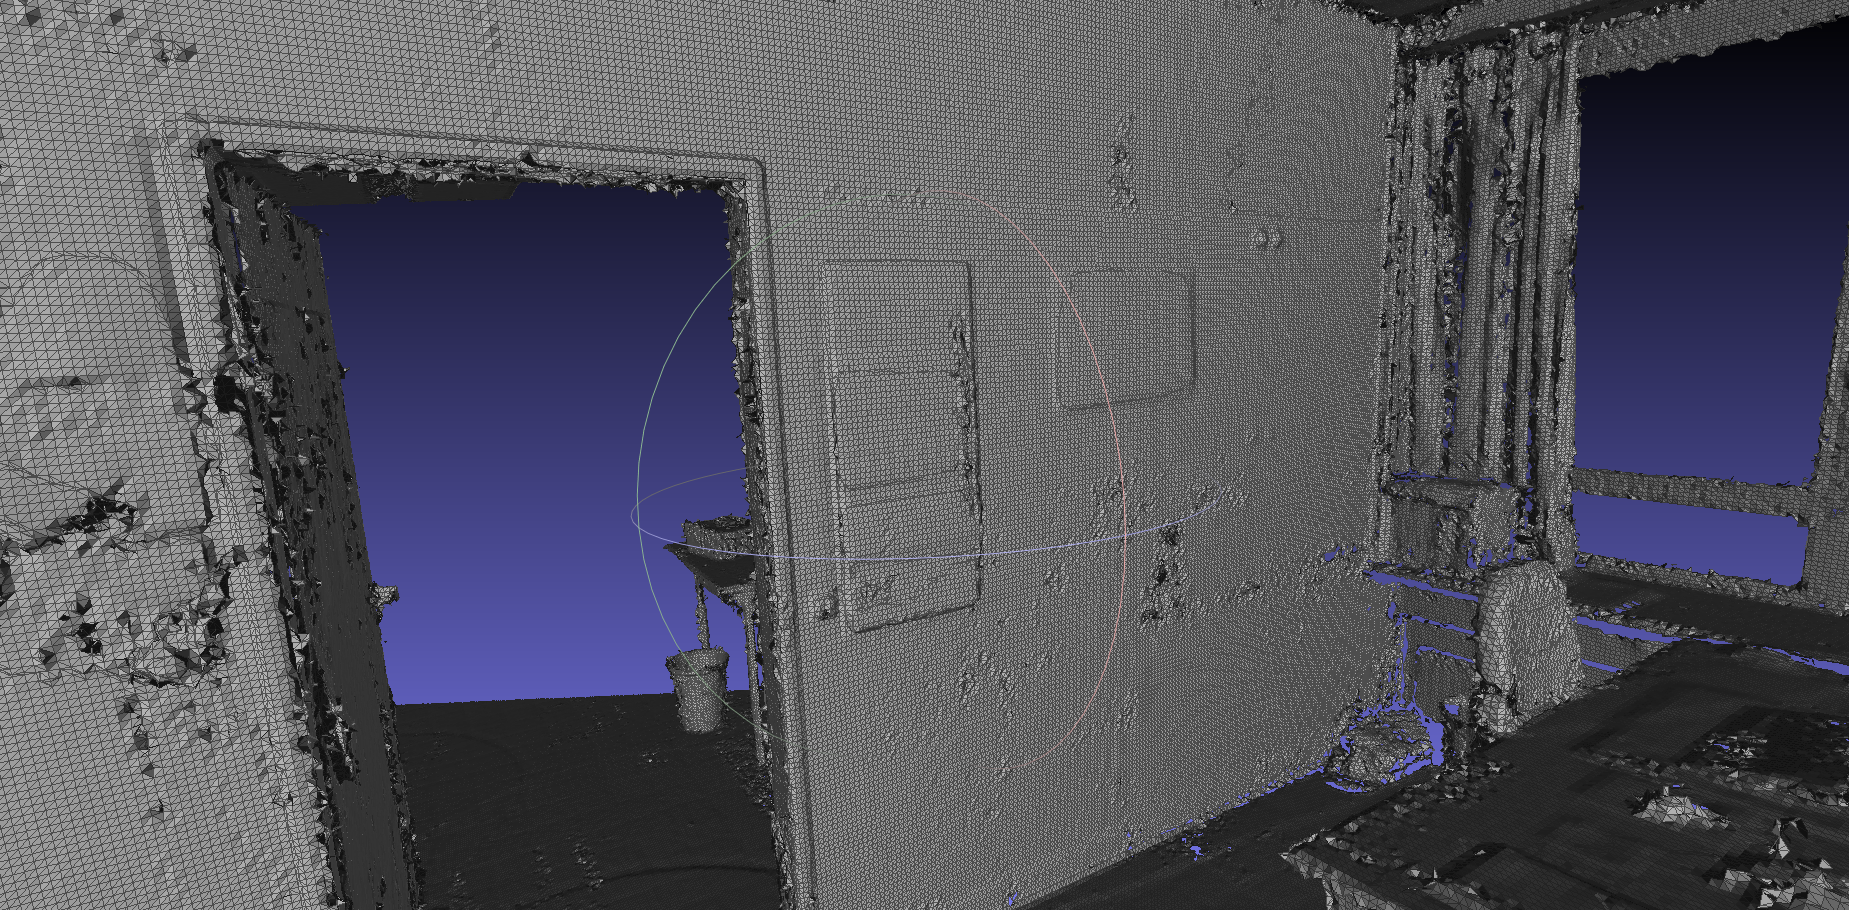
\includegraphics[width=1.0\linewidth]{Images/police_mesh.png}
    \end{figure}
    
    
   \end{column}
  \begin{column}{0.45\textwidth}
  
   \begin{itemize}
    \item Goal: No loss of information with lower memory usage
    \item Reconstruction requires normals of each point
    \item Precalculation of normals in pointset
    \item Calculation of a normal requires nearest neighbors
    
   \end{itemize}
  \end{column}

   
  \end{columns}
 
\end{frame}

\section{Problem Statement}

\subsection*{Nearest Neighbors}
\begin{frame}{Nearest Neighbors}
 
 \begin{itemize}
  \item Undependend searches of nearest neighbors
  \item Calculations of normals for each point based on nearest neighbors
  \item Large runtime for nearest neighbor search on big datasets
  \item Thread based CPU-Implementation in LVR
  \item Idea: GPU-Implementation to reduce runtime
 \end{itemize}

 
\end{frame}

\subsection*{GPU - CPU}
\begin{frame}{GPU - CPU}
 %comparison chart
\end{frame}

\section{Concept and Methods}

\subsection*{CUDA}
\begin{frame}{CUDA}

 \begin{columns}
  
   \begin{column}{0.55\textwidth}
    
  

 \begin{itemize}
  \item Developed by NVIDIA in 2007
  \item Newest version 8.0
  \item API for parallel computing on GPU
  \item C, C++, Fortran, Python
 \end{itemize}
 
  \end{column}
  \begin{column}{0.45\textwidth}
   %NVIDIA CUDA bild klauen
  \end{column}
 \end{columns}


\end{frame}

\begin{frame}{CUDA - Threads}
  \begin{figure}
      \centering
      
      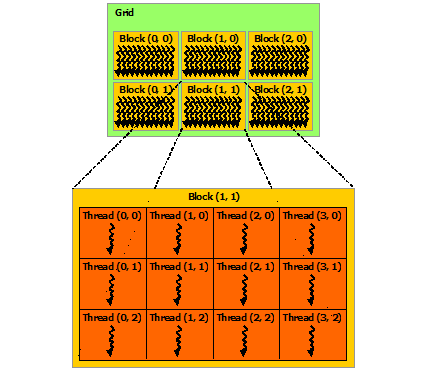
\includegraphics[height=0.7\textheight]{Images/grid-of-thread-blocks.png}
   
    \end{figure}
\end{frame}

\begin{frame}{CUDA - Memory}
   \begin{columns}
  
   \begin{column}{0.4\textwidth}
   
    \begin{figure}
      \centering
   
      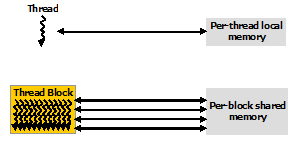
\includegraphics[width=1.0\linewidth]{Images/local_memory.png}
    \end{figure}
    
    
   \end{column}
  \begin{column}{0.6\textwidth}
  
   \begin{figure}
      \centering
   
      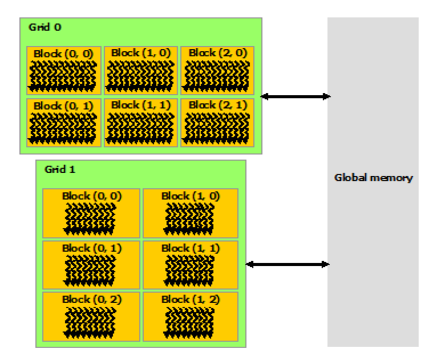
\includegraphics[width=1.0\linewidth]{Images/global_memory.png}
    \end{figure}
  \end{column}

   
  \end{columns}
\end{frame}

\begin{frame}{CUDA - Example}
 % Cuda code von kleinem Beispiel
\end{frame}


\begin{frame}{K Nearest Neighbor Search}
  \begin{columns}[T]
   \begin{column}{0.5\textwidth}
    \textbf{Brute-Force}
    \begin{itemize}
     \item Highly parallelisable
     \item Low memory consumption
     \item Quadric runtime
     \item Asynchron kNN search
     \item Synchron for each point
    \end{itemize}
   \end{column}
  \begin{column}{0.5\textwidth}
    \textbf{Kd-tree}
    
    \begin{itemize}
     \item Only partial parallelisable
     \item Additional memory for tree representation
     \item Approximately linear runtime for low k
     \item Problem of recursion
     \item Asynchron for each point
     \item Synchron kNN search
    \end{itemize}

  \end{column}
  \end{columns}
\end{frame}

\subsection*{Brute-Force}
\begin{frame}{Basic Idea}
 
 %PAP
 
\end{frame}

\begin{frame}{Pseudo-Code}
 
 %pseudo code
 
\end{frame}

\begin{frame}{Distance Calculation}
 % Schneeschaufel: erstes Foto auf Matzes Handy
\end{frame}

\begin{frame}{Sortierung}
 
 %epsilon methode
 %ähnlich wie: https://helloacm.com/wp-content/uploads/2016/03/2012-10-26-knn-concept.png
 %ein vergleich auf allen daten sehr gut parallelisierbar besser als andere sortierungen
 
 
\end{frame}

\subsection*{Kd-tree}
\begin{frame}{Kd-tree}
 
\end{frame}

\begin{frame}{GPU-Implementation}
 
\end{frame}

\begin{frame}{Array based left balanced kd-tree}
 
\end{frame}

\begin{frame}{GPU}
 
\end{frame}

\begin{frame}{Kd-tree search}
 
\end{frame}

\begin{frame}{Kd-tree Knn}
 
\end{frame}

\subsection*{Normal Calculation}
\begin{frame}{Normal Calculation}
 
\end{frame}

\begin{frame}{Normal Flip}
 
\end{frame}

\section{Experiment Results}
\subsection*{Results in LVR-Pipeline}
\begin{frame}{Results in LVR-Pipeline}
 \begin{figure}
  \centering
  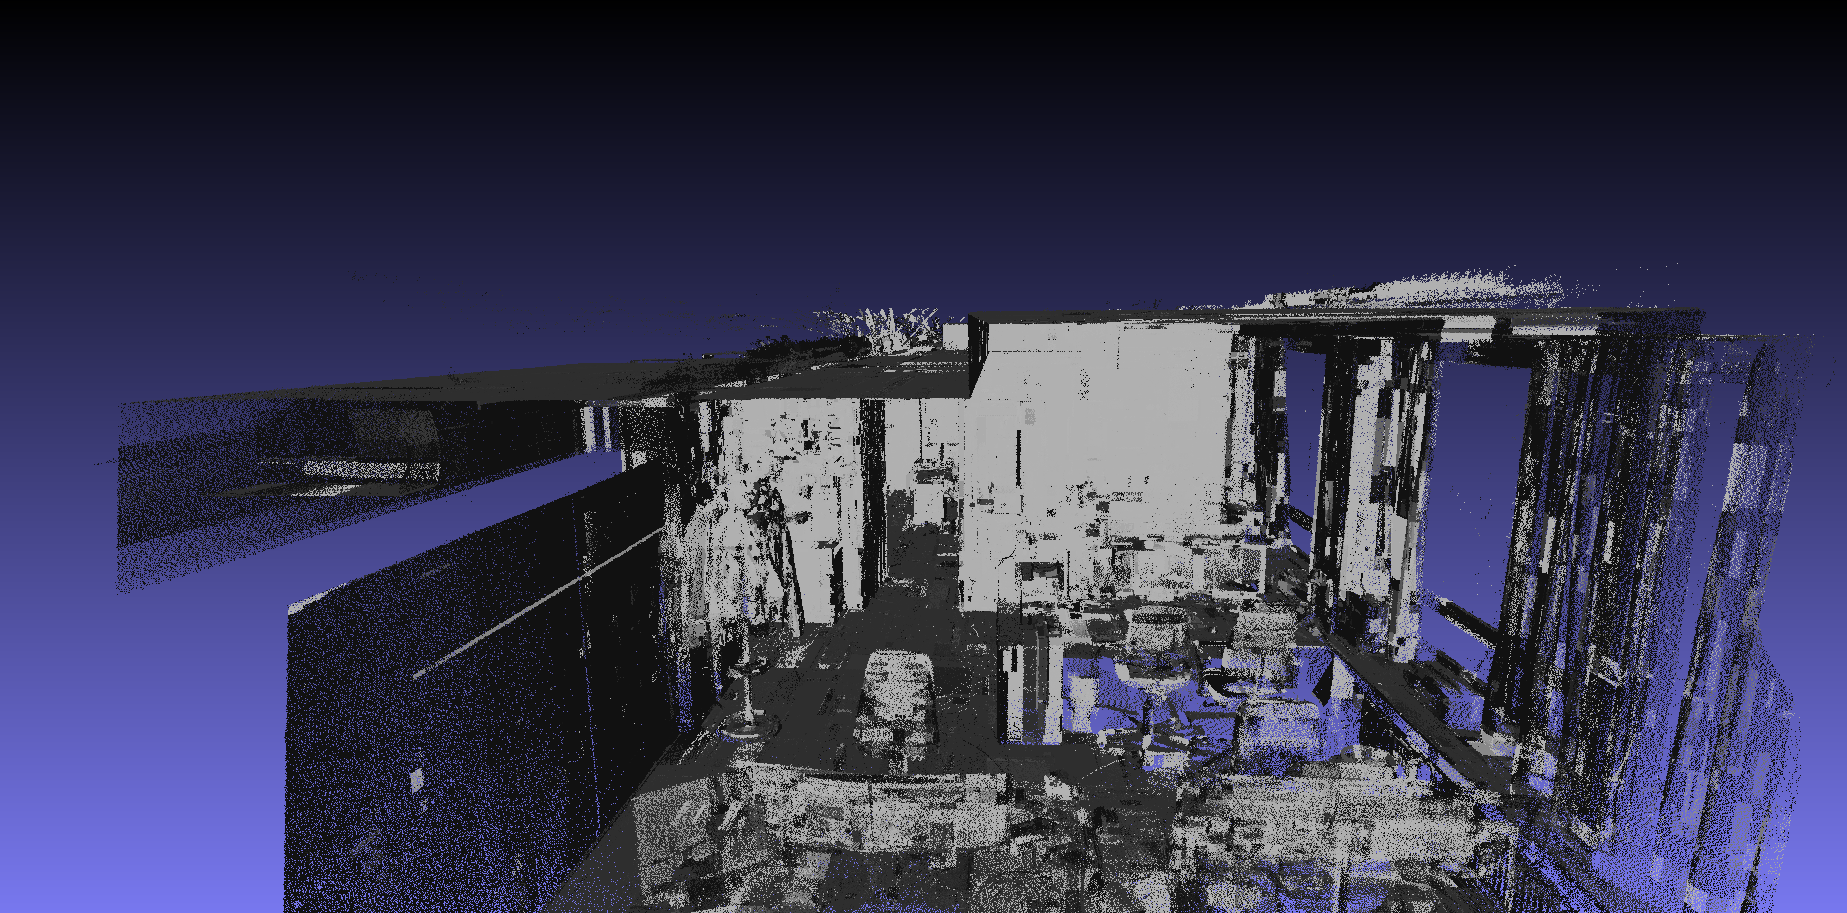
\includegraphics[height=0.4\textheight]{Images/police_no_normals.png}\\
  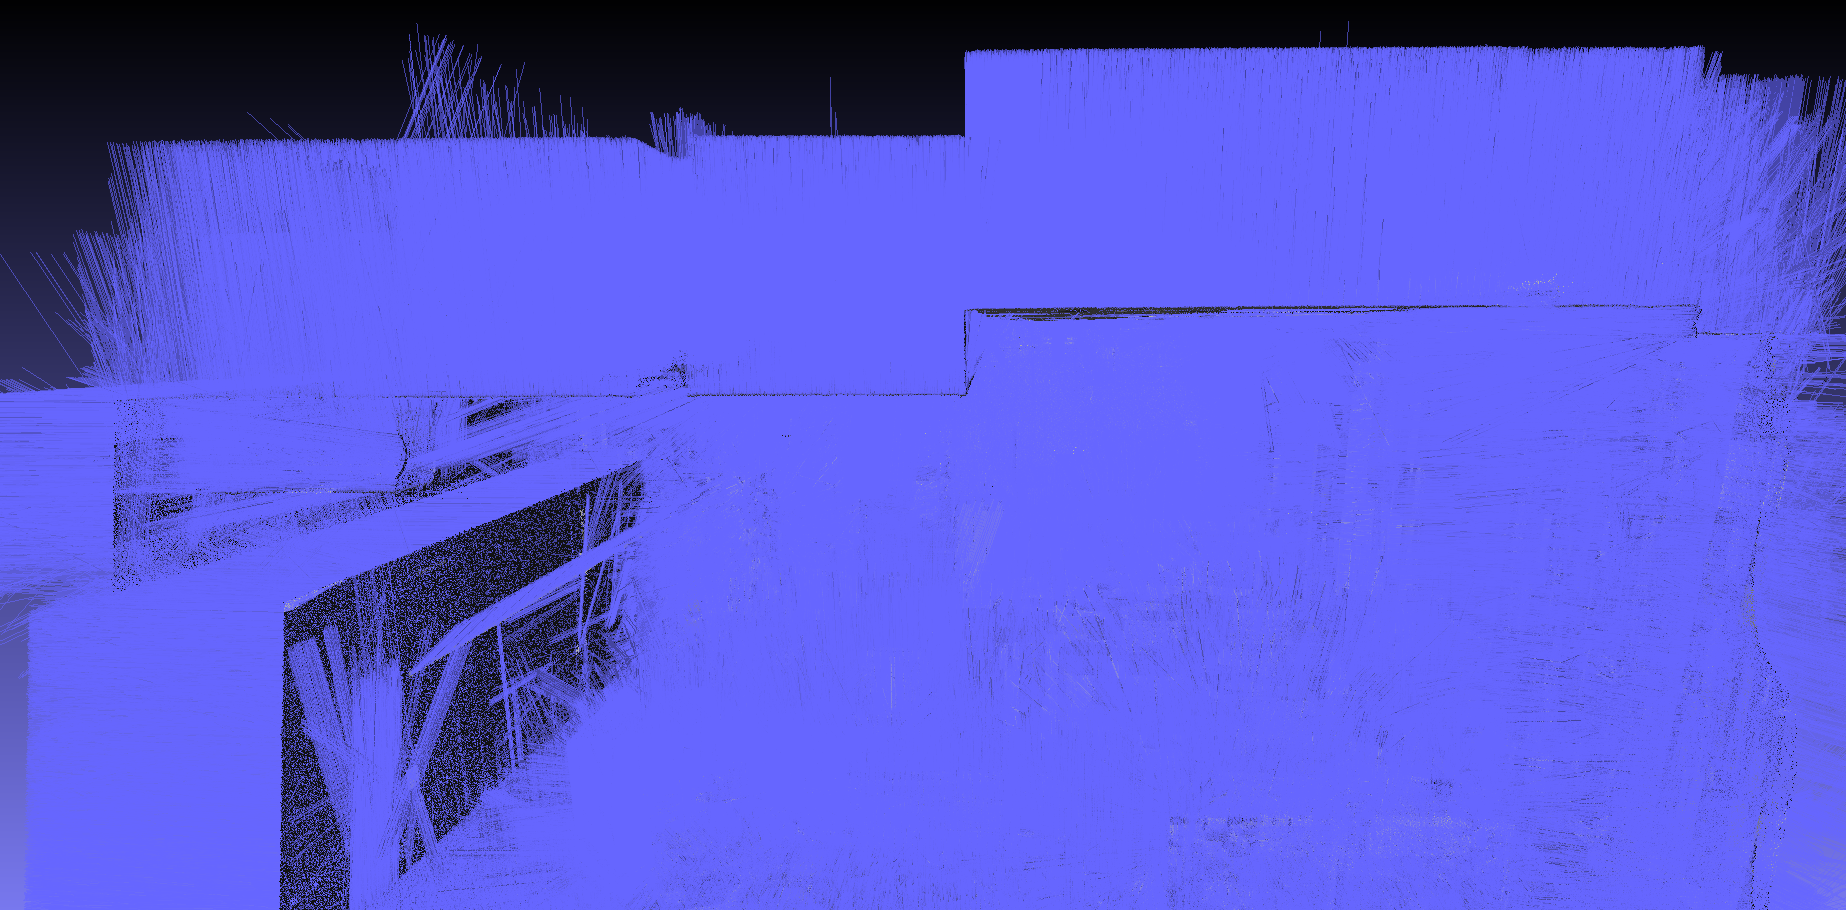
\includegraphics[height=0.4\textheight]{Images/police_normals.png}
 \end{figure}

\end{frame}

\subsection*{Runtime results}
\begin{frame}{Runtime results}
 
\end{frame}

\section{Conclusion}
\begin{frame}{Conclusion}
 
\end{frame}


























\end{document}
